\newpage
\section{Introducción Teórica}\label{sec:introduccion}
\subsection{Colonia de Hormigas}
Es una metaheuristica de la familia de PSO (Particle Swarm Optimization) basada en el comportamiento en grupo de las hormigas para definir el camino a un recurso deseado, en otras palabras es una metodología inspirada en el comportamiento colectivo de las hormigas en su búsqueda de alimentos. 
Es muy usada para soluci\'onar problemas computacionales que pueden reducirse a buscar los mejores caminos o rutas en grafos. Es por eso que es muy importante recordar que las hormigas son prácticamente ciegas, y sin embargo, moviéndose al azar, acaban encontrando el camino más corto desde su nido hasta la fuente de alimentos (y regresar).
Entre sus principales características se encuentran:

\begin{enumerate}
\item Una sola hormiga no es capaz de realizar todo el trabajo sino que termina siendo el resultado de muchas hormigas en conjunto.
\item Una hormiga, cuando se mueve, deja una señal química en el suelo, depositando una sustancia denominada \textbf{feromona}, para que las demás puedan seguirla.
\end{enumerate}

De esta forma, aunque una hormiga aislada se mueva esencialmente al azar, las siguientes decidirán sus movimientos considerando seguir con mayor frecuencia el camino con mayor cantidad de feromonas.

La metaheurística general consiste en lo siguiente:
\begin{enumerate}
\item En principio, todas las hormigas se mueven de manera aleatoria, buscando por si solas un camino al recurso que estan buscando (una posible solución).
\item Una vez encontrada una soluci\'on, la hormiga vuelve, dejando un rastro de feromonas; este rastro puede ser mayor o menor dependiendo de lo buena que sea la solución encontrada. 
\item Utilizando este rastro de feromonas, las hormigas pueden compartir información entre sus distintos pares en la colonia.
\item Cuando una nueva hormiga inicia su trabajo, es influenciada por la feromona depositada por las hormigas anteriores, y así, aumenta las probabilidades de que esta siga los pasos de sus anteriores
al acercarse a un recurso previamente encontrado.
\end{enumerate}


\begin{figure}[h]
\centering
\caption{Ejemplo convergencia a una solución}
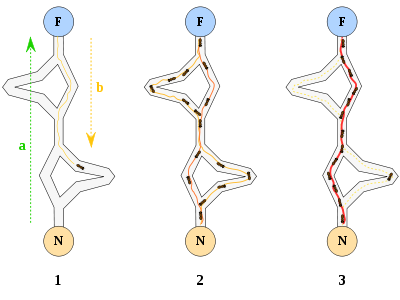
\includegraphics[width=6cm]{imagenes/feromona}
\end{figure}

\begin{figure}[h]
\caption{Ejemplo de uso de feromona}
\centering
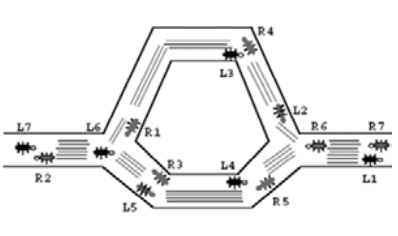
\includegraphics[width=6cm]{imagenes/feromona2}
\end{figure}

En la \textbf{figura 1}, podemos ver una serie de iteraciones donde las hormigas llegan a la Fuente de comida y vuelven, dejando feromonas y en la siguiente iteración la solución se ve influenciada por la feromona. 

Finalmente se llega a una camino, el cual es elegido por casi todas las hormigas, siendo este la soluci\'on final.

En la \textbf{figura 2}, asumiendo que el número de lineas punteadas es proporcional a la cantidad de feromona, se puede ver como el camino inferior es más corto que el superior, por lo cual muchas más hormigas transitarán por éste durante el mismo per\'iodo de tiempo. Esto implica, que en el camino más corto se acumula más feromona mucho más rápido. Después de cierto tiempo, la diferencia en la cantidad de feromona en los dos caminos es lo suficientemente grande para influenciar la decisión de las nuevas hormigas que entren a recorrer estas vías

Se puede ver que una gran ventaja de esta metaheurística es que puede construir una solución intercambiando información entre las distintas hormigas (soluciones), así generar una solución mejor de la que podrían generar individualmente.

Con el paso del tiempo, el rastro de feromonas comienza a evaporarse, y esto produce que los caminos pierdan su fuerza de atracción, cuanto más largo sea el camino, más tiempo demorara una hormiga en recorrerlo, más se evaporará la feromona y por ende serán menos frecuentado. Por su parte los caminos mas cortos (o mas óptimos) tendrán mayor cantidad de feromonas, por ende, mayor probabilidad de ser frecuentados.

ACO fue el primer algoritmo de optimizacion de Colonias de Hormigas desarrollado por Marco Dorigo en su tesis doctoral \cite{paperDorigo}. 

Algunas de las aplicaciones donde se utiliza esta metaheurística:
\begin{enumerate}
\item El problema del viajante de comercio (TSP)
\item Optimización para el diseño de circuitos lógicos combinatorios
\item Problemas de enrutamiento de vehículos
\item Problema de la asignación de horarios
\item Aplicaciones a análisis de ADN y a procesos de producción
\item Partición de un grafo en árboles:
\item Otros
\end{enumerate}



\begin{thebibliography}{9}
\bibitem{wikipedia} 
https://en.wikipedia.org/wiki/Ant\_colony\_optimization\_algorithms

\bibitem{claseMetah} 
http://www-2.dc.uba.ar/materias/metah/meta2016-clase7.pdf

 
\bibitem{paperDorigo} 
http://people.idsia.ch/~gianni/Papers/CEC99.pdf

\bibitem{paperAplicaciones} 
Ant colony optimization: applications and trends. Carlos Algarin

\end{thebibliography}